\documentclass[11pt]{article}
\usepackage[margin=2cm]{geometry}
\usepackage{amsmath,amssymb}
\usepackage{xcolor}
\usepackage{tikz}
\usepackage[backend=biber,style=authoryear]{biblatex}
\addbibresource{bibliography.bib}

\setlength{\parindent}{0pt}
\setlength{\parskip}{0.5\baselineskip}

\title{Astrofísica Moderna\\[0.4em]
\large Transferencia y Procesos Radiativos}
\author{Daniel Soto Villada}
\date{\today}

\begin{document}
\maketitle

\section{Transferencia Radiativa}
\begin{enumerate}
    \item Cuando la profundidad óptica de un medio es $\tau_\nu=0.6$, el medio se considera:
    \begin{itemize}
        \item (A) Ópticamente delgado y prácticamente transparente.
        \item (B) Ópticamente grueso y completamente opaco.
        \item \textcolor{red}{(C) Intermedio (``nublado''), con transmisión parcial.}
        \item (D) Dominado por dispersión más que por absorción.
    \end{itemize}
    \textit{Solución.} La transmisión es $I_\nu/I^0_\nu=e^{-\tau_\nu}$. Para $\tau_\nu=0.6$, la fracción transmitida es $e^{-0.6}\approx0.55$ y la absorbida es $1-e^{-0.6}\approx0.45$. Hay transmisión parcial, por lo que la respuesta es \textbf{(C)}. \parencite[Sec. 13.3.1, pp. 394--395]{chaparro2026}

    \item Un mismo medio puede ser transparente en radio y opaco en ultravioleta porque:
    \begin{itemize}
        \item (A) El índice de refracción cambia con la temperatura.
        \item \textcolor{red}{(B) $\kappa_\nu$ puede variar con la frecuencia.}
        \item (C) Para un mismo $\kappa_\nu$ varía la profundidad óptica $\tau_\nu$.
        \item (D) La longitud de onda de la radiación no influye en la absorción.
    \end{itemize}
    \textit{Solución.} La atenuación depende de $\tau_\nu=\int\kappa_\nu\,ds$. Como el coeficiente de absorción puede depender de la frecuencia, un medio puede tener poca profundidad óptica en radio y mucha en ultravioleta. La respuesta es \textbf{(B)}. \parencite[Secs. 13.2--13.3.1, pp. 390--395]{chaparro2026}

    \item Un haz de intensidad $I_\nu$ atraviesa una lámina infinitesimal de espesor $ds$ en un medio caracterizado por el coeficiente de absorción $\kappa_\nu$. ¿Cuál de las siguientes expresiones representa la fracción de fotones que se pierden (se absorben) en ese trayecto $ds$?
    \begin{itemize}
        \item (A) $\kappa_\nu$
        \item \textcolor{red}{(B) $\kappa_\nu\,ds$}
        \item (C) $I_\nu\kappa_\nu\,ds$
        \item (D) $\dfrac{\kappa_\nu\,ds}{I_\nu}$
    \end{itemize}
    \textit{Solución.} En una lámina sin emisión, $dI_\nu=-\kappa_\nu I_\nu\,ds$. Al dividir por la intensidad incidente, la fracción perdida es $|dI_\nu|/I_\nu=\kappa_\nu\,ds$. La respuesta es \textbf{(B)}. \parencite[Sec. 13.3, pp. 391--394]{chaparro2026}
    \begin{center}
    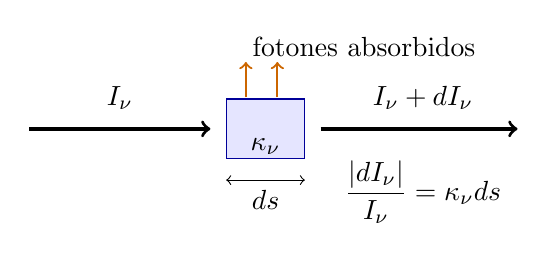
\begin{tikzpicture}[scale=1.0,transform shape]
        \draw[fill=blue!10,draw=blue!60!black] (2.5,-0.38) rectangle (3.5,0.38);
        \node at (3,-0.22) {$\kappa_\nu$};
        \draw[very thick,->] (0,0) -- (2.3,0);
        \node[above] at (1.15,0.12) {$I_\nu$};
        \draw[very thick,->] (3.7,0) -- (6.2,0);
        \node[above] at (5,0.12) {$I_\nu+dI_\nu$};
        \draw[<->] (2.5,-0.65) -- (3.5,-0.65);
        \node[below] at (3,-0.65) {$ds$};
        \draw[->,thick,orange!80!black] (2.75,0.4) -- (2.75,0.85);
        \draw[->,thick,orange!80!black] (3.15,0.4) -- (3.15,0.85);
        \node[above] at (4.25,0.8) {fotones absorbidos};
        \node at (5,-0.8) {$\displaystyle \frac{|dI_\nu|}{I_\nu}=\kappa_\nu ds$};
    \end{tikzpicture}
    \par{\small\textbf{Figura:} Atenuación de un haz al atravesar una lámina infinitesimal.}
    \end{center}

    \item Un gas tenue emite fotones a una razón volumétrica caracterizada por el coeficiente de emisividad $j_\nu$ (energía emitida por unidad de volumen, tiempo, frecuencia y ángulo sólido). Considere una lámina infinitesimal de espesor $ds$ y área unitaria. ¿Cuál expresión representa la energía que la lámina añade a un rayo, por segundo, por Hz y por sr?
    \begin{itemize}
        \item (A) $j_\nu$
        \item (B) $\dfrac{j_\nu}{\kappa_\nu\,ds}$
        \item \textcolor{red}{(C) $j_\nu\,ds$}
        \item (D) $j_\nu I_\nu\,ds$
    \end{itemize}
    \textit{Solución.} La emisividad $j_\nu$ añade intensidad por unidad de recorrido, de modo que en una lámina infinitesimal $dI_\nu=j_\nu\,ds$. La respuesta es \textbf{(C)}. \parencite[Secs. 13.4 y 13.6, pp. 398--402]{chaparro2026}

    \item Según la ecuación general de transferencia radiativa, la intensidad emergente $I_\nu$ será mayor que la incidente $I^0_\nu$ si:
    \begin{itemize}
        \item \textcolor{red}{(A) $j_\nu>I^0_\nu\kappa_\nu$}
        \item (B) $j_\nu<I^0_\nu\kappa_\nu$
        \item (C) $\kappa_\nu=0$
        \item (D) $\tau_\nu\gg1$
    \end{itemize}
    \textit{Solución.} La ecuación local es $dI_\nu/ds=j_\nu-\kappa_\nu I_\nu$. La intensidad aumenta si la emisión supera la absorción; evaluando esta última con la intensidad incidente, se requiere $j_\nu>\kappa_\nu I^0_\nu$. La respuesta es \textbf{(A)}. \parencite[Sec. 13.7, pp. 403--405]{chaparro2026}

    \item En el límite $\tau_\nu\ll1$, con $I^0_\nu=0$, la intensidad emergente se aproxima a:
    \begin{itemize}
        \item \textcolor{red}{(A) $I_\nu\simeq j_\nu L$}
        \item (B) $I_\nu\simeq I^0_\nu e^{-\tau_\nu}$
        \item (C) $I_\nu\simeq S_\nu$
        \item (D) $I_\nu\simeq0$
    \end{itemize}
    \textit{Solución.} Para una fuente uniforme, $I_\nu=S_\nu(1-e^{-\tau_\nu})$. Si $\tau_\nu\ll1$, entonces $1-e^{-\tau_\nu}\approx\tau_\nu$. Usando $S_\nu=j_\nu/\kappa_\nu$ y $\tau_\nu=\kappa_\nu L$, resulta $I_\nu\approx j_\nu L$. La respuesta es \textbf{(A)}. \parencite[Sec. 13.7, pp. 403--405]{chaparro2026}

    \item En un medio no homogéneo, $\kappa_\nu(s)$ podría aumentar con la profundidad. ¿Qué pasa si asumiéramos (incorrectamente) que $S_\nu$ es constante respecto a $s$?
    \begin{itemize}
        \item (A) Se sobreestima la emisión total.
        \item \textcolor{red}{(B) Se subestima la emisión total.}
        \item (C) No afecta el resultado.
        \item (D) Hace que $I_\nu$ sea independiente de $\tau_\nu$.
    \end{itemize}
    \textit{Solución.} Bajo la interpretación de que $j_\nu$ es constante y se aproxima $S_\nu=j_\nu/\kappa_\nu$ por su valor en la cara más profunda, la función fuente real es mayor en las capas más superficiales. La solución formal, midiendo $t$ desde la cara del observador hacia el interior, es
    \[
        I_{\nu,\mathrm{out}}=I^0_\nu e^{-\tau_{\nu,\mathrm{tot}}}
        +\int_0^{\tau_{\nu,\mathrm{tot}}}S_\nu(t)e^{-t}\,dt.
    \]
    Como $S_\nu(t)\geq S_{\nu,\mathrm{deep}}$ en las capas superficiales, reemplazarla por el valor profundo reduce la integral de emisión a $S_{\nu,\mathrm{deep}}(1-e^{-\tau_{\nu,\mathrm{tot}}})$. Así, se subestima la contribución emitida y la intensidad emergente; corresponde la opción \textbf{(B)}. Sin especificar qué valor constante se adopta para $S_\nu$, el enunciado original no determina por sí solo el sentido del error. \parencite[Sec. 13.7, pp. 403--405]{chaparro2026}

    \item Una estrella tipo T Tauri intrínsecamente emite el mismo flujo en el visible ($\lambda_1=0.5\,\mu\mathrm{m}$) y en el infrarrojo cercano ($\lambda_2=1.0\,\mu\mathrm{m}$). Sin embargo, está rodeada de polvo que sigue una ley de extinción $A_\lambda\propto\lambda^{-1}$. Las observaciones muestran que el brillo a $0.5\,\mu\mathrm{m}$ se atenúa en 5 magnitudes y el flujo a $1.0\,\mu\mathrm{m}$ es dos veces mayor que el flujo esperado de la estrella. ¿Cuál explicación reconcilia ambas observaciones?
    \begin{itemize}
        \item (A) La extinción es igual en todas las longitudes de onda; el exceso IR se debe a variabilidad intrínseca de la estrella.
        \item \textcolor{red}{(B) $A_{1\,\mu\mathrm{m}}\simeq2.5\,\mathrm{mag}$; el polvo absorbe energía en visible/UV y la reemite en el IR.}
        \item (C) $A_{1\,\mu\mathrm{m}}\simeq0\,\mathrm{mag}$; la luz visible absorbida se dispersa sin calentar el polvo y el exceso IR proviene de líneas del gas.
        \item (D) $A_{1\,\mu\mathrm{m}}\simeq-5\,\mathrm{mag}$; el exceso IR es un artefacto instrumental.
    \end{itemize}
    \textit{Solución.} La ley de extinción da $A_{1\,\mu\mathrm{m}}=5(0.5/1.0)=2.5\,\mathrm{mag}$. La luz estelar directa se atenúa por un factor $10^{-0.4(2.5)}=0.1$; el exceso infrarrojo se explica por la reemisión térmica del polvo que absorbió radiación de longitudes de onda cortas. La respuesta es \textbf{(B)}. \parencite[Secs. 12.2--12.3 y 14.8.7, pp. 375--383, 469--470]{chaparro2026}
    \begin{center}
    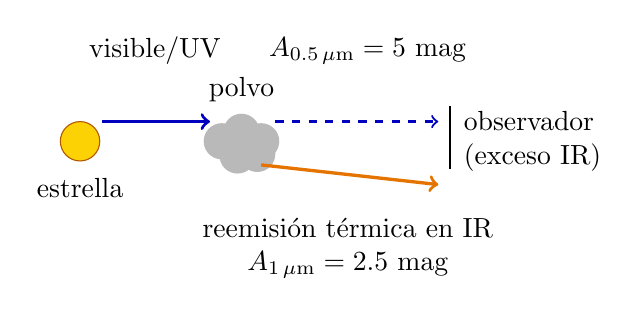
\begin{tikzpicture}[scale=1.0,transform shape]
        \draw[fill=yellow!70!orange,draw=orange!70!black] (0,0) circle (0.25);
        \node[below] at (0,-0.35) {estrella};
        \draw[very thick,->,blue!75!black] (0.28,0.25) -- (1.65,0.25);
        \node[above] at (0.95,0.85) {visible/UV};
        \foreach \x/\y in {1.8/0,2.05/0.12,2.3/0,2.0/-0.18,2.25/-0.16} {
            \fill[gray!55] (\x,\y) circle (0.23);
        }
        \node[above] at (2.05,0.38) {polvo};
        \draw[->,thick,blue!75!black,dashed] (2.48,0.25) -- (4.55,0.25);
        \node[above] at (3.65,0.85) {$A_{0.5\,\mu\mathrm{m}}=5$ mag};
        \draw[->,very thick,orange!90!black] (2.3,-0.3) -- (4.55,-0.55);
        \node[below,align=center] at (3.4,-0.85) {reemisión térmica en IR\\$A_{1\,\mu\mathrm{m}}=2.5$ mag};
        \draw[thick] (4.7,-0.35) -- (4.7,0.45);
        \node[right,align=left] at (4.75,0) {observador\\(exceso IR)};
    \end{tikzpicture}
    \par{\small\textbf{Figura:} El polvo atenúa la luz estelar directa y reemite en el infrarrojo la energía absorbida.}
    \end{center}

    \item ¿Cuál conjunto de parámetros describe mejor un disco rico en polvo iluminado por una estrella (comparado con una nebulosa aislada y difusa) en longitudes de onda IR?
    \begin{itemize}
        \item (A) $\kappa_\nu$ bajo, $j_\nu$ bajo.
        \item (B) $\kappa_\nu$ bajo, $j_\nu$ alto.
        \item (C) $\kappa_\nu$ alto, $j_\nu$ bajo.
        \item \textcolor{red}{(D) $\kappa_\nu$ alto, $j_\nu$ alto.}
    \end{itemize}
    \textit{Solución.} Un disco rico en polvo tiene abundante material absorbente, por lo que $\kappa_\nu$ es alto. Al estar iluminado por una estrella, el polvo se calienta y su emisividad infrarroja $j_\nu$ también es alta. La respuesta es \textbf{(D)}. \parencite[Secs. 13.4 y 14.8.7--14.8.8, pp. 398, 469--470]{chaparro2026}

    \item En meteorología se adopta como umbral de visibilidad la distancia a la que la profundidad óptica cumple $\tau\simeq3$. ¿Cuál es la distancia máxima de visibilidad correspondiente? (Pista: un coeficiente $\kappa=0.015\,\mathrm{m}^{-1}$ corresponde a una distancia de 200 m.)
    \begin{itemize}
        \item \textcolor{red}{(A) $s=3/\kappa$}
        \item (B) $s=3\kappa$
        \item (C) $s=e^{-3}$
        \item (D) Faltan datos.
    \end{itemize}
    \textit{Solución.} Para un medio uniforme, $\tau=\kappa s$, así que $s=\tau/\kappa=3/(0.015\,\mathrm{m}^{-1})=200\,\mathrm{m}$. La respuesta es \textbf{(A)}. \parencite[Secs. 13.3.1 y 13.3.3, pp. 394--396]{chaparro2026}

    \item Se observa una fuente puntual ($F^*_\nu$) en el mismo campo de visión que una fuente resuelta y difusa ($I^{\mathrm{sky}}_\nu$), dentro de un mismo haz $\Omega$ de un telescopio. La luz pasa primero a través de un gas tibio ($T_w,\tau_w$) y luego por un gas frío ($T_c,\tau_c$). ¿Cuál expresión describe correctamente el flujo observado?
    \begin{itemize}
        \item \textcolor{red}{(A)}
        {\color{red}
        \[
        \begin{aligned}
        &[F^*_\nu+I^{\mathrm{sky}}_\nu\Omega]e^{-(\tau_c+\tau_w)}\\
        &\quad+\Omega\left[B_\nu(T_w)(1-e^{-\tau_w})e^{-\tau_c}
        +B_\nu(T_c)(1-e^{-\tau_c})\right].
        \end{aligned}
        \]}
        \item (B)
        \[
        \begin{aligned}
        &[F^*_\nu+I^{\mathrm{sky}}_\nu\Omega]e^{-(\tau_c+\tau_w)}\\
        &\quad+\Omega\left[B_\nu(T_c)(1-e^{-\tau_c})e^{-\tau_w}
        +B_\nu(T_w)(1-e^{-\tau_w})\right].
        \end{aligned}
        \]
        \item (C)
        \[
        \begin{aligned}
        &[I^{\mathrm{sky}}_\nu\Omega]e^{-(\tau_c+\tau_w)}\\
        &\quad+\Omega\left[B_\nu(T_w)(1-e^{-\tau_w})e^{-\tau_c}
        +B_\nu(T_c)(1-e^{-\tau_c})\right].
        \end{aligned}
        \]
        \item (D)
        \[
        \begin{aligned}
        &[I^{\mathrm{sky}}_\nu\Omega]e^{-(\tau_c+\tau_w)}\\
        &\quad+\Omega\left[B_\nu(T_c)(1-e^{-\tau_c})e^{-\tau_w}
        +B_\nu(T_w)(1-e^{-\tau_w})\right].
        \end{aligned}
        \]
        \end{itemize}
    \textit{Solución.} La emisión de la capa tibia se atenúa al atravesar la capa fría, mientras que la emisión de esta última llega directamente al observador. Por ello,
    \[
        F_{\nu,\mathrm{obs}}=(F^*_\nu+I^{\mathrm{sky}}_\nu\Omega)e^{-(\tau_w+\tau_c)}
        +\Omega B_\nu(T_w)(1-e^{-\tau_w})e^{-\tau_c}
        +\Omega B_\nu(T_c)(1-e^{-\tau_c}),
    \]
    que corresponde a la opción \textbf{(A)}. \parencite[Secs. 13.6--13.7, pp. 400--405]{chaparro2026}
    \begin{center}
    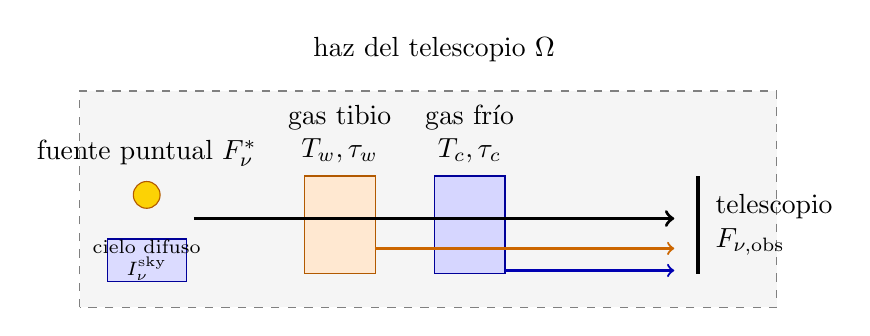
\begin{tikzpicture}[scale=1.0,transform shape]
        \fill[gray!8] (-4.5,-1.05) rectangle (4.35,1.7);
        \draw[dashed,gray] (-4.5,-1.05) rectangle (4.35,1.7);
        \node[above] at (0,1.95) {haz del telescopio $\Omega$};
        \draw[fill=yellow!70!orange,draw=orange!70!black] (-3.65,0.38) circle (0.17);
        \node[above] at (-3.65,0.62) {fuente puntual $F^*_\nu$};
        \draw[fill=blue!14,draw=blue!60!black] (-4.15,-0.72) rectangle (-3.15,-0.18);
        \node[font=\scriptsize,align=center] at (-3.65,-0.45) {cielo difuso\\$I^{\mathrm{sky}}_\nu$};
        \draw[fill=orange!18,draw=orange!70!black] (-1.65,-0.62) rectangle (-0.75,0.62);
        \node[above,align=center] at (-1.2,0.66) {gas tibio\\$T_w,\tau_w$};
        \draw[fill=blue!16,draw=blue!60!black] (0,-0.62) rectangle (0.9,0.62);
        \node[above,align=center] at (0.45,0.66) {gas frío\\$T_c,\tau_c$};
        \draw[very thick,->] (-3.05,0.08) -- (3.05,0.08);
        \draw[->,thick,orange!80!black] (-0.75,-0.3) -- (3.05,-0.3);
        \draw[->,thick,blue!70!black] (0.9,-0.58) -- (3.05,-0.58);
        \draw[very thick] (3.35,-0.62) -- (3.35,0.62);
        \node[right,align=left] at (3.45,0) {telescopio\\$F_{\nu,\mathrm{obs}}$};
    \end{tikzpicture}
    \par{\small\textbf{Figura:} Las fuentes de fondo atraviesan primero el gas tibio y luego el frío antes de llegar al telescopio.}
    \end{center}
\end{enumerate}

\subsection{Cálculos}
\begin{enumerate}
    \item Para un gas con $\kappa_\nu=0.25\,\mathrm{cm}^{-1}$ y $L=8\,\mathrm{cm}$, considerando una intensidad incidente $I^0_\nu=5\times10^{-8}\,\mathrm{Jy\,sr^{-1}}$ y sin emisión interna ($S_\nu=0$), la intensidad emergente es:
    \begin{itemize}
        \item (A) $4.5\times10^{-8}\,\mathrm{Jy\,sr^{-1}}$
        \item (B) $1.8\times10^{-8}\,\mathrm{Jy\,sr^{-1}}$
        \item \textcolor{red}{(C) $6.8\times10^{-9}\,\mathrm{Jy\,sr^{-1}}$}
        \item (D) $1.3\times10^{-9}\,\mathrm{Jy\,sr^{-1}}$
    \end{itemize}
    \textit{Solución.} La profundidad óptica es $\tau_\nu=\kappa_\nu L=(0.25)(8)=2$. Como no hay emisión interna, $I_{\nu,\mathrm{out}}=I^0_\nu e^{-\tau_\nu}=(5\times10^{-8})e^{-2}=6.77\times10^{-9}\,\mathrm{Jy\,sr^{-1}}$. Redondeando, la respuesta es \textbf{(C)}, $6.8\times10^{-9}\,\mathrm{Jy\,sr^{-1}}$. \parencite[Secs. 13.3.1 y 13.7, pp. 394--395, 403--405]{chaparro2026}

    \item Una estrella de fondo aporta $I^0_\nu=10\,\mathrm{mJy/beam}$ a través de una capa con $\kappa_\nu=0.4\,\mathrm{pc}^{-1}$, $j_\nu/\kappa_\nu=7\,\mathrm{mJy/beam}$ y $L=1\,\mathrm{pc}$. La intensidad emergente es:
    \begin{itemize}
        \item (A) $7.5\,\mathrm{mJy/beam}$
        \item \textcolor{red}{(B) $9.0\,\mathrm{mJy/beam}$}
        \item (C) $11.2\,\mathrm{mJy/beam}$
        \item (D) $16.8\,\mathrm{mJy/beam}$
    \end{itemize}
    \textit{Solución.} Aquí $\tau_\nu=\kappa_\nu L=0.4$ y $S_\nu=j_\nu/\kappa_\nu=7\,\mathrm{mJy/beam}$. Entonces,
    \[
        I_{\nu,\mathrm{out}}=I^0_\nu e^{-\tau_\nu}+S_\nu(1-e^{-\tau_\nu})
        =10e^{-0.4}+7(1-e^{-0.4})\approx9.01\,\mathrm{mJy/beam}.
    \]
    La respuesta es \textbf{(B)}, $9.0\,\mathrm{mJy/beam}$. \parencite[Secs. 13.6--13.7, pp. 400--405]{chaparro2026}

    \item La extinción en magnitudes y la profundidad óptica se relacionan mediante
    \[
        A_\nu=(2.5\log_{10}e)\tau_\nu\simeq1.086\tau_\nu.
    \]
    En una línea de visión a través de una nube se mide $A_\nu=2.17\,\mathrm{mag}$. Si el medio es homogéneo y la función fuente es constante, la solución de la ecuación de transferencia radiativa es $I_\nu=S_\nu(1-e^{-\tau_\nu})$. ¿Qué fracción de $S_\nu$ alcanza al observador?
    \begin{itemize}
        \item \textcolor{red}{(A) $0.87S_\nu$}
        \item (B) $0.50S_\nu$
        \item (C) $0.14S_\nu$
        \item (D) $0.01S_\nu$
    \end{itemize}
    \textit{Solución.} De $A_\nu=1.086\tau_\nu$ se obtiene $\tau_\nu=2.17/1.086\approx2.00$. Por tanto,
    \[
        I_\nu=S_\nu(1-e^{-\tau_\nu})\approx S_\nu(1-e^{-2})\approx0.865S_\nu\approx0.87S_\nu.
    \]
    La respuesta es \textbf{(A)}. \parencite[Secs. 13.3.1--13.3.2 y 13.7, pp. 394--395, 403--405]{chaparro2026}
\end{enumerate}

\section{Procesos Radiativos}
\begin{enumerate}
    \item Un telescopio cuyo límite de magnitud observable es 30 puede ver estrellas $X$ veces menos brillantes que el límite de magnitud típico del ojo humano en el cielo nocturno ($\approx5$). ¿Cuánto vale $X$?
    \begin{itemize}
        \item (A) $X=5$
        \item (B) $X=15$
        \item (C) $X=200$
        \item \textcolor{red}{(D) $X=10^{10}$}
    \end{itemize}
    \textit{Solución.} La relación entre magnitud y flujo es $m_1-m_2=-2.5\log_{10}(F_1/F_2)$. La diferencia entre el límite del ojo y el del telescopio es $30-5=25$ magnitudes, por lo que
    \[
        X=\frac{F_{\mathrm{ojo}}}{F_{\mathrm{tel}}}=10^{0.4(25)}=10^{10}.
    \]
    El telescopio detecta fuentes cien mil millones de veces más débiles que el ojo, de modo que la opción correcta es \textbf{(D)}. \parencite{chaparro2026}

    \item Si la distancia $d$ a un objeto se expresa en Mpc, ¿cuál es la expresión correcta para el módulo de distancia?
    \begin{itemize}
        \item \textcolor{red}{(A) $m-M=5\log_{10}(d)+25$}
        \item (B) $m-M=5\log_{10}(d)-5$
        \item (C) $m-M=5\log_{10}(d)+5$
        \item (D) $m-M=5\log_{10}(d)+11$
    \end{itemize}
    \textit{Solución.} Con la distancia en parsecs, el módulo de distancia es $m-M=5\log_{10}(d_{\mathrm{pc}})-5$. Como $d_{\mathrm{pc}}=10^6d_{\mathrm{Mpc}}$, se obtiene
    \[
        m-M=5\log_{10}(10^6d_{\mathrm{Mpc}})-5=5\log_{10}(d_{\mathrm{Mpc}})+25.
    \]
    La opción correcta es \textbf{(A)}. \parencite{chaparro2026}

    \item HD 122563 tiene una luminosidad de $340L_\odot$ y Groombridge 1618 tiene una luminosidad de $0.15L_\odot$. Calcule la proporción entre sus radios, asumiendo que ambas tienen la misma temperatura ($T\approx4200\,\mathrm{K}$).
    \begin{itemize}
        \item (A) $R_{\mathrm{HD}}/R_{\mathrm{Groom}}\approx1$
        \item \textcolor{red}{(B) $R_{\mathrm{HD}}/R_{\mathrm{Groom}}\approx48$}
        \item (C) $R_{\mathrm{HD}}/R_{\mathrm{Groom}}\approx340$
        \item (D) $R_{\mathrm{HD}}/R_{\mathrm{Groom}}\approx2260$
    \end{itemize}
    \textit{Solución.} Por la ley de Stefan--Boltzmann, $L=4\pi R^2\sigma T^4$. Al tener ambas estrellas la misma temperatura, $L\propto R^2$ y
    \[
        \frac{R_{\mathrm{HD}}}{R_{\mathrm{Groom}}}
        =\sqrt{\frac{L_{\mathrm{HD}}}{L_{\mathrm{Groom}}}}
        =\sqrt{\frac{340}{0.15}}\approx47.6\approx48.
    \]
    La opción correcta es \textbf{(B)}. \parencite{chaparro2026}

    \item HD 122563 tiene una luminosidad de $340L_\odot$ y Groombridge 1618 tiene una luminosidad de $0.15L_\odot$. Ambas tienen la misma masa ($M\approx0.8M_\odot$). Si $L\propto M^{3.5}$, ¿qué explica que ambas tengan la misma temperatura ($T\approx4200\,\mathrm{K}$) pero distinta luminosidad?
    \begin{itemize}
        \item (A) HD está en la secuencia principal y Groombridge no.
        \item \textcolor{red}{(B) Groombridge está en la secuencia principal y HD no.}
        \item (C) HD es una enana blanca.
        \item (D) No son ejemplos realistas; es imposible que tengan la misma masa y temperatura.
    \end{itemize}
    \textit{Solución.} La relación masa--luminosidad $L\propto M^{3.5}$ describe aproximadamente estrellas de la secuencia principal. Groombridge 1618 es compatible con una estrella de baja luminosidad de secuencia principal; HD 122563, con luminosidad mucho mayor a masa y temperatura similares, es una estrella evolucionada fuera de la secuencia principal. De $L=4\pi R^2\sigma T^4$, a igual temperatura la diferencia de luminosidad implica radios distintos. La opción correcta es \textbf{(B)}. \parencite{chaparro2026}

    \item Supongamos que la temperatura de Júpiter es $T=110\,\mathrm{K}$ y su radio aproximado es $R=7.15\times10^7\,\mathrm{m}$. Encuentre su luminosidad.
    \begin{itemize}
        \item (A) $5.3\times10^{17}L_\odot$
        \item \textcolor{red}{(B) $1.4\times10^{-9}L_\odot$}
        \item (C) $4\times10^{-3}L_\odot$
        \item (D) $10L_\odot$
    \end{itemize}
    \textit{Solución.} Modelando a Júpiter como un emisor térmico, $L=4\pi R^2\sigma T^4$. En unidades solares,
    \[
        \frac{L}{L_\odot}=\left(\frac{R}{R_\odot}\right)^2
        \left(\frac{T}{T_\odot}\right)^4
        \approx\left(\frac{7.15\times10^7}{6.96\times10^8}\right)^2
        \left(\frac{110}{5772}\right)^4\approx1.4\times10^{-9}.
    \]
    La opción correcta es \textbf{(B)}. \parencite{chaparro2026}

    \begin{samepage}
    \item Una estrella tiene un exceso de color $E_{B-V}=0.05$. Asumiendo un coeficiente de extinción de $2\,\mathrm{mag\,kpc^{-1}}$, ¿a qué distancia se encuentra?
    \begin{itemize}
        \item (A) $2\,\mathrm{kpc}$
        \item (B) $180\,\mathrm{pc}$
        \item \textcolor{red}{(C) $78\,\mathrm{pc}$}
        \item (D) $10\,\mathrm{pc}$
    \end{itemize}
    \textit{Solución.} Suponiendo el valor típico $R_V=A_V/E_{B-V}\approx3.1$, la extinción visual es $A_V\approx3.1(0.05)=0.155\,\mathrm{mag}$. Con una tasa de extinción de $2\,\mathrm{mag\,kpc^{-1}}$,
    \[
        d\approx\frac{A_V}{2\,\mathrm{mag\,kpc^{-1}}}
        =0.0775\,\mathrm{kpc}\approx78\,\mathrm{pc}.
    \]
    La opción correcta es \textbf{(C)}. Sin asumir un valor para $R_V$, el exceso de color por sí solo no determina $A_V$. \parencite{chaparro2026}
    \end{samepage}

    \item Una estrella similar al Sol tiene $(B-V)_0=0.7$ y un exceso de color $E_{B-V}=0.05$. ¿Dónde está el pico observado de $B_\lambda$?
    \begin{itemize}
        \item (A) $120\,\mathrm{nm}$
        \item (B) $400\,\mathrm{nm}$
        \item (C) $502\,\mathrm{nm}$
        \item \textcolor{red}{(D) $550\,\mathrm{nm}$}
    \end{itemize}
    \textit{Solución.} El color observado es $(B-V)=(B-V)_0+E_{B-V}=0.70+0.05=0.75$. La aproximación color--temperatura para una estrella similar al Sol da $T_{\mathrm{eff}}\approx5.3\times10^3\,\mathrm{K}$; por la ley de desplazamiento de Wien, $\lambda_{\max}=2.898\times10^{-3}\,\mathrm{m\,K}/T_{\mathrm{eff}}\approx5.5\times10^{-7}\,\mathrm{m}=550\,\mathrm{nm}$. La opción correcta es \textbf{(D)}. \parencite{chaparro2026}

    \item Una región del medio interestelar contiene granos de polvo con un coeficiente de absorción lineal $\kappa_\nu=6.0\times10^{-22}\,\mathrm{cm^{-1}}$ a cierta frecuencia $\nu$. Asumiendo que el medio es uniforme, calcule el coeficiente de extinción en magnitudes por kpc.
    \begin{itemize}
        \item (A) $a_\nu\approx0.0001\,\mathrm{mag\,kpc^{-1}}$
        \item (B) $a_\nu\approx0.02\,\mathrm{mag\,kpc^{-1}}$
        \item (C) $a_\nu\approx1\,\mathrm{mag\,kpc^{-1}}$
        \item \textcolor{red}{(D) $a_\nu\approx2\,\mathrm{mag\,kpc^{-1}}$}
    \end{itemize}
    \textit{Solución.} En $1\,\mathrm{kpc}=3.086\times10^{21}\,\mathrm{cm}$, la profundidad óptica es
    \[
        \tau_\nu=\kappa_\nu d=(6.0\times10^{-22})(3.086\times10^{21})\approx1.85.
    \]
    Como $A_\nu=1.086\tau_\nu$, el coeficiente de extinción es $a_\nu\approx1.086(1.85)\approx2.0\,\mathrm{mag\,kpc^{-1}}$. La opción correcta es \textbf{(D)}. \parencite{chaparro2026}

    \item Un contenedor cúbico transparente de 10 cm de lado contiene un gas a $T=3500\,\mathrm{K}$. El gas se ilumina por detrás con una fuente cuya intensidad a $1\,\mathrm{GHz}$ es $I^0_\nu=2\times10^{-15}\,\mathrm{erg\,s^{-1}\,cm^{-2}\,Hz^{-1}\,sr^{-1}}$. Si el coeficiente de absorción del gas a esa frecuencia es $0.01\,\mathrm{cm^{-1}}$, ¿qué intensidad mide un detector al otro lado del gas?
    \begin{itemize}
        \item \textcolor{red}{(A) $I^0_\nu e^{-\kappa_\nu L}+B_\nu(T)(1-e^{-\kappa_\nu L})$}
        \item (B) $B_\nu(T)(1-e^{-\kappa_\nu L})$
        \item (C) $I^0_\nu+B_\nu(T)$
        \item (D) $I^0_\nu e^{-\kappa_\nu L}$
    \end{itemize}
    \textit{Solución.} La profundidad óptica es $\tau_\nu=\kappa_\nu L=(0.01)(10)=0.1$. Para el gas en equilibrio térmico, la solución es
    \[
        I_{\nu,\mathrm{out}}=I^0_\nu e^{-\tau_\nu}+B_\nu(T)(1-e^{-\tau_\nu}).
    \]
    A $1\,\mathrm{GHz}$ y $3500\,\mathrm{K}$ se cumple el régimen de Rayleigh--Jeans, de modo que $B_\nu(T)\approx2kT\nu^2/c^2\approx1.07\times10^{-15}\,\mathrm{erg\,s^{-1}\,cm^{-2}\,Hz^{-1}\,sr^{-1}}$. Así,
    \[
        I_{\nu,\mathrm{out}}\approx1.91\times10^{-15}\,\mathrm{erg\,s^{-1}\,cm^{-2}\,Hz^{-1}\,sr^{-1}}
        \approx1.9\times10^8\,\mathrm{Jy\,sr^{-1}}.
    \]
    La opción correcta es \textbf{(A)}. \parencite{chaparro2026}

    \item Dos capas sucesivas tienen parámetros $(\tau_1,S_{1,\nu})$ y $(\tau_2,S_{2,\nu})$; no hay intensidad incidente ($I_{\nu,0}=0$). Encuentre la intensidad emergente $I_{\nu,\mathrm{out}}$ y evalúe para $\tau_1=0.5$, $S_{1,\nu}=2$, $\tau_2=1.2$ y $S_{2,\nu}=6$ (unidades arbitrarias).
    {\small
    \begin{itemize}
        \item (A) $I_{\nu,\mathrm{out}}=S_{1,\nu}(1-e^{-\tau_1})(1-e^{-\tau_2})+S_{2,\nu}(1-e^{-\tau_2})$
        \item (B) $I_{\nu,\mathrm{out}}=S_{1,\nu}(1-e^{-\tau_1})+S_{2,\nu}(1-e^{-\tau_2})$
        \item (C) $I_{\nu,\mathrm{out}}=S_{2,\nu}(1-e^{-\tau_2})e^{-\tau_1}+S_{1,\nu}(1-e^{-\tau_1})$
        \item \textcolor{red}{(D) $I_{\nu,\mathrm{out}}=S_{1,\nu}(1-e^{-\tau_1})e^{-\tau_2}+S_{2,\nu}(1-e^{-\tau_2})$}
    \end{itemize}}
    \textit{Solución.} La primera capa emite $S_{1,\nu}(1-e^{-\tau_1})$; al pasar por la segunda capa, esta contribución se atenúa por $e^{-\tau_2}$. La segunda capa añade $S_{2,\nu}(1-e^{-\tau_2})$. Por tanto,
    \[
        I_{\nu,\mathrm{out}}=S_{1,\nu}(1-e^{-\tau_1})e^{-\tau_2}
        +S_{2,\nu}(1-e^{-\tau_2}).
    \]
    Sustituyendo los valores dados, $I_{\nu,\mathrm{out}}=2(1-e^{-0.5})e^{-1.2}+6(1-e^{-1.2})\approx4.43$. La opción correcta es \textbf{(D)}. \parencite{chaparro2026}
\end{enumerate}

\section{Electromagnetismo}
\begin{enumerate}
    \item Según la fórmula de Larmor,
    \[
        P=\frac{q^2a^2}{6\pi\varepsilon_0c^3},
    \]
    ¿cuál de las siguientes partículas emite radiación electromagnética?
    \begin{itemize}
        \item (A) Un electrón en reposo en el laboratorio.
        \item (B) Un electrón que se mueve en línea recta con velocidad constante $v=0.99c$.
        \item \textcolor{red}{(C) Un electrón que describe una circunferencia con rapidez constante.}
        \item (D) Un protón que se mueve en línea recta con velocidad constante.
    \end{itemize}
    \textit{Solución.} La potencia de Larmor es proporcional a $a^2$, por lo que una carga radia cuando está acelerada. El electrón que describe una circunferencia tiene aceleración centrípeta $a=v^2/r$, aunque su rapidez sea constante; las partículas con velocidad constante no radian. La opción correcta es \textbf{(C)}. \parencite{chaparro2026}

    \item Una carga que se movía con velocidad $v_0$ frena bruscamente en un tiempo muy corto $t_0$. Un tiempo $T\gg t_0$ después, dentro de la esfera de radio $R=cT$ el campo eléctrico apunta a la posición actual de la carga; fuera de ella, apunta a la posición donde estaría si no hubiera frenado. ¿Qué ocurre en el cascarón de grosor $ct_0$ que separa ambas regiones?
    \begin{itemize}
        \item (A) Las líneas de campo son puramente radiales y el cascarón no transporta energía.
        \item \textcolor{red}{(B) Las líneas conectan ambas regiones: aparece una componente tangencial $E_t$ que viaja a $c$ como un pulso electromagnético.}
        \item (C) La región exterior se entera del frenado de inmediato y se reorganiza alrededor de la nueva posición de la carga.
        \item (D) El campo eléctrico se anula por completo dentro del cascarón.
    \end{itemize}
    \textit{Solución.} La información sobre el frenado se propaga a velocidad finita, $c$. Por eso, el campo lejano aún refleja el movimiento previo, mientras que el campo cercano ya responde al estado posterior. La transición ocurre en el cascarón y contiene una componente tangencial del campo eléctrico, acompañada por un campo magnético: es un pulso electromagnético que transporta energía. La opción correcta es \textbf{(B)}. \parencite{chaparro2026}

    \item Un electrón oscila verticalmente a lo largo de $\hat{z}$ y radia con
    \[
        \frac{dP}{d\Omega}=\frac{q^2a^2}{16\pi^2\varepsilon_0c^3}\sin^2\theta,
    \]
    donde $\theta$ se mide desde $\hat{z}$. ¿Dónde debemos ubicar un detector (siempre a la misma distancia del electrón) para captar la señal más intensa?
    \begin{itemize}
        \item (A) Justo encima del electrón ($\theta=0$).
        \item (B) Justo debajo del electrón ($\theta=\pi$).
        \item (C) En $\theta=\pi/4$.
        \item \textcolor{red}{(D) En el plano horizontal que pasa por el electrón ($\theta=\pi/2$).}
    \end{itemize}
    \textit{Solución.} A distancia fija, la potencia por unidad de ángulo sólido es proporcional a $\sin^2\theta$. Esta función alcanza su máximo cuando $\theta=\pi/2$, es decir, en el plano perpendicular a la aceleración del electrón. La opción correcta es \textbf{(D)}. \parencite{chaparro2026}

    \item Un electrón y un protón (misma carga en magnitud) se aceleran libremente bajo el mismo campo eléctrico $E$. ¿Cuál es aproximadamente el cociente $P_e/P_p$ de las potencias que radian? Use $m_p/m_e\approx1836$.
    \begin{itemize}
        \item (A) $P_e/P_p=1$
        \item (B) $P_e/P_p\approx1.8\times10^3$
        \item \textcolor{red}{(C) $P_e/P_p\approx3.4\times10^6$}
        \item (D) $P_e/P_p\approx3.0\times10^{-7}$
    \end{itemize}
    \textit{Solución.} Para cada partícula, $a=|q|E/m$. Como $P\propto q^2a^2$, y las cargas tienen igual magnitud, $P\propto m^{-2}$. Por tanto,
    \[
        \frac{P_e}{P_p}=\left(\frac{m_p}{m_e}\right)^2
        =1836^2\approx3.37\times10^6\approx3.4\times10^6.
    \]
    La opción correcta es \textbf{(C)}. \parencite{chaparro2026}

    \item En su marco de reposo $S$, dos placas paralelas muy extensas con densidades $\pm\sigma$ producen entre ellas un campo $E=\sigma/\varepsilon_0$ perpendicular a las placas. Un observador $S'$ se mueve con $v=0.6c$ respecto a $S$. ¿Qué campo $E'$ mide entre las placas si se mueve (i) perpendicular a las placas o (ii) paralelo a ellas?
    \begin{itemize}
        \item (A) (i) $E'=E$; (ii) $E'=E$.
        \item \textcolor{red}{(B) (i) $E'=E$; (ii) $E'=1.25E$.}
        \item (C) (i) $E'=1.25E$; (ii) $E'=E$.
        \item (D) (i) $E'=0.80E$; (ii) $E'=1.25E$.
    \end{itemize}
    \textit{Solución.} Para movimiento perpendicular a las placas, la velocidad es paralela al campo eléctrico, cuya componente paralela permanece invariante: $E'_{\parallel}=E$. Para movimiento paralelo a las placas, la velocidad es perpendicular al campo, y $E'_{\perp}=\gamma E$, donde
    \[
        \gamma=\frac{1}{\sqrt{1-v^2/c^2}}=\frac{1}{\sqrt{1-0.6^2}}=1.25.
    \]
    Así, los resultados son (i) $E'=E$ y (ii) $E'=1.25E$. La opción correcta es \textbf{(B)}. \parencite{chaparro2026}

    \item Una carga puntual está en reposo en $S$: allí solo hay un campo eléctrico radial y $\mathbf{B}=0$. Un observador $S'$ se mueve con velocidad $\mathbf{v}$ respecto a $S$. En $S'$ (con las direcciones paralela y perpendicular medidas respecto a $\mathbf{v}$):
    \begin{itemize}
        \item \textcolor{red}{(A) $E'_{\parallel}=E_{\parallel}$ y $E'_{\perp}=\gamma E_{\perp}$; el campo ya no es esférico y aparece un campo magnético $\mathbf{B}'$.}
        \item (B) El campo eléctrico es idéntico al de $S$ y no hay campo magnético, porque $\mathbf{E}$ es invariante entre marcos.
        \item (C) $E'_{\parallel}=\gamma E_{\parallel}$ y $E'_{\perp}=E_{\perp}$, sin campo magnético en $S'$.
        \item (D) El campo eléctrico desaparece y solo se observa un campo magnético, porque en $S'$ la carga se mueve.
    \end{itemize}
    \textit{Solución.} Las transformaciones de campos separan las componentes respecto a la velocidad: $E'_{\parallel}=E_{\parallel}$ y, dado que $\mathbf{B}=0$ en $S$, $E'_{\perp}=\gamma E_{\perp}$. Además, el movimiento relativo mezcla los campos y produce un campo magnético $\mathbf{B}'$ no nulo. La distribución eléctrica deja de ser esféricamente simétrica en $S'$. La opción correcta es \textbf{(A)}. \parencite{chaparro2026}

    \item Una placa infinita con densidad superficial de carga $\sigma$, en reposo en $S$, produce $E=\sigma/(2\varepsilon_0)$ y $B=0$. Un observador $S'$ se mueve con $v=0.6c$ paralelo a la placa. En $S'$ las cargas forman una hoja de corriente $K'=\sigma'v$, con $\sigma'=\gamma\sigma$, que produce $B'=\mu_0K'/2$. ¿Cuánto mide $|B'|$? Use $\mu_0\varepsilon_0=1/c^2$.
    \begin{itemize}
        \item (A) $B'=0$, porque en $S$ no hay campo magnético.
        \item (B) $B'=0.60E/c$
        \item \textcolor{red}{(C) $B'=0.75E/c$}
        \item (D) $B'=1.25E/c$
    \end{itemize}
    \textit{Solución.} Usando $\sigma'=\gamma\sigma$ y $K'=\sigma'v$,
    \[
        B'=\frac{\mu_0K'}{2}=\frac{\mu_0\gamma\sigma v}{2}.
    \]
    Como $E=\sigma/(2\varepsilon_0)$ y $\mu_0\varepsilon_0=1/c^2$, resulta $B'=\gamma(v/c)E/c$. Para $v=0.6c$, $\gamma=1.25$ y $\gamma v/c=0.75$, de modo que $B'=0.75E/c$. La opción correcta es \textbf{(C)}. \parencite{chaparro2026}

    \item Un alambre neutro lleva una corriente $I$: en el laboratorio, cargas positivas (separación $\ell$) se mueven con velocidad $v$ y un número igual de cargas negativas (separación $\ell$) están en reposo. Una carga de prueba $Q$ se mueve paralela al alambre con la misma velocidad $v$ y siente una fuerza magnética $QvB$. En el marco de $Q$ (donde $Q$ está en reposo), esta fuerza:
    \begin{itemize}
        \item (A) Es nula: una carga en reposo no siente fuerza magnética y el alambre sigue siendo neutro.
        \item \textcolor{red}{(B) Es eléctrica: por la contracción de longitudes ($\ell_-\ne\ell_+$), el alambre adquiere carga neta.}
        \item (C) Sigue siendo magnética y de la misma magnitud $QvB$.
        \item (D) Es una fuerza ficticia, pues $Q$ está en reposo.
    \end{itemize}
    \textit{Solución.} En el marco que se mueve con las cargas positivas, estas quedan en reposo, mientras que las negativas se mueven y sus separaciones se contraen: $\ell'_- =\ell/\gamma$, frente a la separación propia de las positivas $\ell'_+=\gamma\ell$. Así, las densidades lineales dejan de compensarse y el alambre adquiere carga neta. La fuerza sobre $Q$, ahora en reposo, es eléctrica en ese marco. La opción correcta es \textbf{(B)}. \parencite{chaparro2026}

    \item Dos cargas iguales $q$ están en reposo en $S$, separadas una distancia $r$ perpendicular a $\mathbf{v}$; la fuerza entre ellas es $F=q^2/(4\pi\varepsilon_0r^2)$. En el laboratorio $S'$ ambas se mueven en paralelo con rapidez $v=0.6c$. La transformación de fuerzas da una fuerza total $F'_{\perp}=F/\gamma$, pero la transformación de campos da una fuerza eléctrica $qE'_{\perp}=\gamma F$. La discrepancia se explica por la fuerza magnética entre las cargas en movimiento. ¿Cuánto vale el cociente $F'_{\mathrm{mag}}/F'_{\mathrm{el}}$?
    \begin{itemize}
        \item (A) $0$
        \item (B) $0.60$
        \item (C) $1.25$
        \item \textcolor{red}{(D) $0.36$}
    \end{itemize}
    \textit{Solución.} La fuerza magnética se opone a la eléctrica, así que $F'_{\mathrm{mag}}=F'_{\mathrm{el}}-F'_{\perp}$. Con $F'_{\mathrm{el}}=\gamma F$ y $F'_{\perp}=F/\gamma$,
    \[
        \frac{F'_{\mathrm{mag}}}{F'_{\mathrm{el}}}
        =1-\frac{1}{\gamma^2}=\frac{v^2}{c^2}=(0.6)^2=0.36.
    \]
    La opción correcta es \textbf{(D)}. \parencite{chaparro2026}

    \item En $S$ hay un campo magnético uniforme $\mathbf{B}=B\hat{y}$ y ningún campo eléctrico. Un observador $S'$ se mueve con $\mathbf{v}=0.6c\hat{x}$. Con las transformaciones
    \[
        \mathbf{E}'_{\perp}=\gamma(\mathbf{E}_{\perp}+\mathbf{v}\times\mathbf{B}),
        \qquad
        \mathbf{B}'_{\perp}=\gamma\left(\mathbf{B}_{\perp}-\frac{\mathbf{v}\times\mathbf{E}_{\perp}}{c^2}\right),
    \]
    ¿qué campos mide $S'$?
    \begin{itemize}
        \item \textcolor{red}{(A) $|\mathbf{E}'|=0.75cB$ y $|\mathbf{B}'|=1.25B$.}
        \item (B) $|\mathbf{E}'|=0$ y $|\mathbf{B}'|=B$.
        \item (C) $|\mathbf{E}'|=0.60cB$ y $|\mathbf{B}'|=B$.
        \item (D) $|\mathbf{E}'|=0.75cB$ y $|\mathbf{B}'|=0.80B$.
    \end{itemize}
    \textit{Solución.} Como $\mathbf{E}=0$, las transformaciones dan $\mathbf{E}'=\gamma(\mathbf{v}\times\mathbf{B})$ y $\mathbf{B}'=\gamma\mathbf{B}$. Aquí $\mathbf{v}\perp\mathbf{B}$, de modo que
    \[
        |\mathbf{E}'|=\gamma vB=(1.25)(0.6)cB=0.75cB,
        \qquad |\mathbf{B}'|=\gamma B=1.25B.
    \]
    La opción correcta es \textbf{(A)}. \parencite{chaparro2026}
\end{enumerate}

\printbibliography[title={Referencias}]

\end{document}